\documentclass[9pt,twoside]{pnas-new}
\usepackage{booktabs}
\usepackage{float}
% Use the lineno option to display guide line numbers if required.
\setboolean{displaywatermark}{false}

\articletype{SOCIAL SCIENCES}%%%% Article topic/classification

\templatetype{pnasmathematics} % Choose template
% {pnasresearcharticle} = Template for a two-column research article
% {pnasmathematics} = Template for a one-column mathematics article
% {pnasinvited} = Template for a PNAS invited submission
%\onecolumn

\begin{document}

\title{Gotham FC's Move to Queens: Does transit accessibility translate to attendance?}

% Use letters for affiliations, numbers to show equal authorship (if applicable) and to indicate the corresponding author
\author[a,1]{Isabel Prado-Tucker}

\affil[a]{Quantitative Social Science,
Dartmouth College, Hanover, NH 03755}

% Please give the surname of the lead author for the running footer
\leadauthor{Prado-Tucker}

% Please add a significance statement to explain the relevance of your work
\significancestatement{ 
The growth of the National Women's Soccer League (NWSL) is about much more than soccer in the United States; it signals increased investment in women's sports globally, and the development of a new fan that is shifting media economics. Gotham FC's move from Harrison, NJ to Queens, NY reflects this exactly. The move will nearly triple the number of people who can reach the stadium in an hour, positioning Gotham in the largest NWSL market with the greatest transit accessibility of any team stadium. But will this unprecedented accessibility meaningfully increase Gotham's attendance? We ran predictive models and synthetic control to make an estimate.}

\authorcontributions{I.P.T. designed the research, built the isochrone and modeling pipeline, and wrote the paper.}
\authordeclaration{The author declares no competing interest.}
\correspondingauthor{\textsuperscript{1}Email: isabel.a.prado-tucker.28@dartmouth.edu}
% Please include corresponding author, author contribution and author declaration information
% \authorcontributions{Please provide details of author contributions here.}
% \authordeclaration{Please declare any competing interests here.}
% \equalauthors{\textsuperscript{1}A.O.(Author One) contributed equally to this work with A.T. (Author Two) (remove if not applicable).}
% \correspondingauthor{\textsuperscript{2}To whom correspondence should be addressed. E-mail: author.two\@email.com}

% At least three keywords are required at submission. Please provide three to five keywords, separated by the pipe symbol.
\keywords{National Women's Soccer League $|$ New York City $|$ Sports Attendance $|$  Public Transportation Accessibility}

\begin{abstract}
Gotham FC of the National Women's Soccer League (NWSL) is relocating from Sports Illustrated Stadium in Harrison, NJ to Etihad Park in Queens in 2028, nearly tripling its 60-minute transit catchment population, from 1.05 million to 3.20 million people. Gotham ranks among the lowest third of the league in average attendance despite representing the largest metro area. This paper asks whether that accessibility gain will meaningfully increase attendance. I fit a linear model of log(attendance) on log(catchment population), clustered by team, then trained a CatBoost model on its residual using 950 team-games and all other features because a standard tree model cannot extrapolate past the accessibility range it saw in training. Both stages were evaluated with Leave-One-Venue-Out (LOVO) cross-validation, and the predicted shift to Etihad Park was decomposed with SHAP. A synthetic-control model built from eight non-relocating teams was validated on Seattle Reign and Washington Spirit, which already relocated. All models agree accessibility is among the largest positive predictors of attendance (coefficient 0.177, p=0.038), and the single largest driver of the predicted Etihad Park shift. Three comparable relocations gained 69 to 174 percent post-move, and Gotham's 2028 attendance is projected between 14,962 and 22,849 fans (60 to 91 percent of capacity) once league-wide growth is separated out. That being said, every model struggled to generalize to an unfamiliar venue, and while transit accessibility is very likely a key driver of Gotham's predicted gain, there is insufficient data to pin down how strong that effect is.
\end{abstract}

\dates{This manuscript was compiled on \today}
\doi{\url{www.pnas.org/cgi/doi/10.1073/pnas.XXXXXXXXXX}}

\maketitle
\thispagestyle{firststyle}
\ifthenelse{\boolean{shortarticle}}{\ifthenelse{\boolean{singlecolumn}}{\abscontentformatted}{\abscontent}}{}


\Firstpage
\section{Introduction}
The National Women's Soccer League (NWSL) commenced its inaugural season in 2013, after the former women's professional league in the United States folded in 2012. In light of this context, as the league began, it faced significant skepticism from players, fans, and the media as to whether it could survive long-term.

Attendance and expansion fee records are broken regularly in the NWSL. Earlier this season, the attendance record was shattered, with 63,004 fans watching new expansion team Denver Summit FC play the Washington Spirit. The trend seems clear: the NWSL is in a period of rapid growth; however, some are more skeptical about whether the league is set up for long-term success.

Gotham FC represents New Jersey and New York, and in 2028 is moving from Sports Illustrated Stadium in Harrison, NJ to the new Etihad Park in Willets Point, Queens, which it will share with NYCFC. This move will strengthen the team's New York City identity and make games accessible to more fans. The team's July, 2026 game at Citi Field (across the street from Etihad Park) drew 42,175 fans, which is well above the team's current home game average of 8,110 fans. 
\Endparasplit Since the National Women's Soccer League is relatively new and has much less data availability than men's leagues, most of the research on machine learning models for predicting sports attendance focuses on men's leagues. There are two main competing theories about where a team should relocate. The first school of thought argues for prioritizing market-access, to maximize the number of people who can easily reach the stadium. The suburban penalty has been documented in the NWSL, meaning attendance declines by about 6.6 percent for every mile an NWSL team is from their city center \cite{DoesLocationMatterAnEconometricAnalysisofStadiumLocationandAttendanceatNationalWomensSoccerLeagueMatches}. The enclosure model argues the opposite. A study on the NFL argued that franchises have a strong economic incentive to separate themselves from businesses to force attendees to remain in the stadium and spend more money \cite{mls}. This manifests as stadiums in suburban areas surrounded by a moat of parking lots. The NWSL's smaller crowds and younger fan-base make the market-access model the more plausible of the two, but it has never been tested against a relocation that changes accessibility by a factor of three. There's a third mechanism at play here: the honeymoon effect, where attendance increases by up to 20 percent within 5 years of a stadium's opening, regardless of accessibility increases \cite{article}. 

Other known attendance factors in the NWSL include weather, team quality, star players, USWNT activity, and seating capacity \cite{doi:10.1177/15270025231217973}. The superstar effect can be substantial: games involving Caitlin Clark accounted for roughly half of the WNBA's league-wide attendance growth in her rookie year \cite{clarkonomics}, and a similar but smaller effect has been identified in the NWSL for star players such as Alex Morgan and Sam Kerr \cite{doi:10.1177/15270025231217973}. Capacity constraints complicate measuring attendance effect. One study controlled for capacity's effect on attendance using Tobit regression \cite{DoesLocationMatterAnEconometricAnalysisofStadiumLocationandAttendanceatNationalWomensSoccerLeagueMatches}. Most capacity-constrained NWSL games occur at KC Current's stadium—the first built specifically for a women's professional sports team—whose capacity is well below the league average.

Given these confounds, I test three predictions. First, catchment population is positively associated with attendance across the league. Second, if access rather than novelty drives the lift, accessibility remains the dominant contributor even after venue, schedule, weather, and team-quality features are controlled. Third, across relocations, the size of the attendance lift tracks the size of the accessibility gain.
Both modeling strategies used have precedent. A recent study on Major League Soccer found XGBoost to outperform linear regression and random forest models \cite{Beermann25012026}. In other sport's attendance studies, CatBoost and XGBoost are roughly equivalent and treated as the gold standard, so CatBoost is used here for the ease of handling categorical features \cite{articleCatBoost}. Synthetic control has been used to model the effects of NFL expansion on local job markets, and the effects of MLB stadium relocation on property value \cite{repec:sae:jospec:v:20:y:2019:i:2:p:242-260} \cite{repec:spr:ecogov:v:23:y:2022:i:3:d:10.1007_s10101-022-00268-z}. Neither study applies synthetic control to attendance, however, which is the gap this paper works in.


\section{Data}
\subsection{Soccer Game, Match, Stadium, and Player Data} Game-, team-season, and stadium-level data come from the sister project, \textit{What Drives NWSL Attendance: Evidence of a Durable, Women’s Specific Sports Culture} which pulled data from the American Soccer Analysis (ASA) API via the \textit{itscalledsoccer} Python wrapper. The NWSL began in 2013, but the ASA only started reliably reporting attendance data in 2016, so the first three seasons (2013-2015) are excluded from every attendance analysis in this paper. The unit of analysis in the original ASA datasets are the individual matches, teams, and stadiums. This project uses team-game data of 1,132 home games (2016-2019, 2022-2026) for the linear stage, the CatBoost residual stage, and the SHAP mechanism check; the synthetic control instead uses a team-season panel (14 x 9) of NWSL attendance over the same window. Missing stadium name, location, and capacity fields were scraped from Wikipedia and NWSL/MLS metro-center coordinates were built by hand into a lookup table. 2020 and 2021 are excluded from every attendance model in this paper because attendance was severely restricted during the COVID-19 pandemic. Washington Spirit and Gotham both relocated in 2021, so it is necessary to consider the COVID-context when analyzing their stadium relocations. The main challenge is not missing values, but the size of the datasets. There are 1,132 team-games, and 4 recent stadium relocations. It is difficult to extrapolate a model with that small a sample size to an entirely new stadium with unprecedented accessibility. Another limitation is that Kansas City Current moved to the first purpose-built women's soccer stadium, but their attendance is capacity-constrained at nearly every game. Therefore, Kansas City is removed from the CatBoost training set and the synthetic-control comparison set because its attendance reflects the stadium's small capacity, not true demand. 

\subsection{Transit Feeds and Maps} General Transit Feed Specification (GTFS) schedule data and Open Street Map (OSM) pedestrian/road networks were pulled the metro area of all 14 NWSL teams who have more than one completed season, including the four most recent stadium relocations (Kansas City, Seattle, San Diego, Washington) and Gotham's own upcoming move. This data is later used to build transit isochrones around the NWSL stadiums.

\subsection{Census information} 2020 Census tract geometries and American Community Survey (ACS) population and demographic (income, race/ethnicity) data was pulled for every census tract within the defined isochrones and joined to isochrone travel times to build reachable-population and demographic-shift numbers at the tract level.

\section{Methods}
\subsection{Spatial data and isochrome build}
For each metro area, r5py was used to build a transit and walk network from the respective metro's GTFS feed(s) and clipped OSM extract to define travel-time isochrones from each stadium at 30, 45, 60, and 90-minute thresholds. Every isochrone is set on Saturday at 6 pm, which is a standard time for a game, but may not capture true transit variability within individual markets. Each isochrone was then spatially joined to census tract geometries, where a tract was counted as reachable if its centroid falls inside the isochrone polygon, and reachable-population values were computed by summing ACS population data across the included tracts. By default, r5py sets the walking speed at 3.6 km/hr, which is significantly slower than the standard walking speed of 5 km/hr used by Google Maps. I confirmed this with a itinerary on a real route, Sports Illustrated Stadium to the Harrison PATH station, and a 1,000 meter path took 16:44 at the default speed versus roughly 12 minutes at a more realistic pace, so I updated every isochrone to match the standard 5.0 km/hr estimate. The correction significantly increased Sports Illustrated Stadium's 60-minute reachable population from 620,000 to 1.05 million, in large part due to increased accessibility from Manhattan. 

\subsection{Linear accessibility}
\begin{equation}
\log(\text{attendance}_{i}) = \beta_0 + \beta_1 \log(\text{catchment\_population}_{v(i)}) + \varepsilon_{i}, \quad \varepsilon_i \; \text{clustered by team}
\label{eq:linear}
\end{equation}
Originally, accessibility (the number of people who can reach the stadium in 60 minutes, based on the isochrones) was a standard feature in the CatBoost model, but CatBoost could not extrapolate based on Etihad Park's unprecedented 3.2 million person reach. The linear stage regresses log(attendance) on log(catchment\_population), the 60-minute isochrone catchment population, with standard errors clustered by team, on the 950 of 1,132 team-games with a non-missing catchment value (older venues without isochrones are dropped for the linear stage but still used in CatBoost because it can handle null values). Etihad's raw catchment is 2.2 times larger than any value in the training set, so the predictor is log-transformed, making Etihad only 0.78 units past the observed maximum. Extrapolating by less than one unit in log-scale is much more reasonable than the 2.2x raw catchment increase. The in-sample fit and Leave-One-Venue-Out (LOVO) cross-validation were both computed. For LOVO, I hold one team-venue pair out at a time, train the model on every other pair, and then pool together every held out group's predictions. This is in place of a Leave-One-Team-Out design because Gotham is an established team, just relocating to a novel stadium. This cross-validation allows us to interpret how well these models can predict Gotham's attendance in Etihad Park.

\subsection{CatBoost attendance model}
A CatBoostRegressor (depth 6, 300 iterations, learning rate 0.05, L2 leaf regularization 3, chosen by a 24-combination grid search scored against pooled LOVO $R^2$) was fit on the residual left over from the linear stage, \begin{equation}
\text{residual}_i = \log(\text{attendance}_i) - \widehat{\text{linear\_pred}}_i
\label{eq:residual},
\end{equation} using every feature except catchment population itself, which includes running table rank, opponent table rank, days since last home game, day of week, year, venue name, home team, away team, stadium capacity, points per game, points back from the current playoff line, game-day maximum temperature and precipitation (from the Open-Meteo Archive API,), the venue's home-city share of commuters who use public transit (ACS table B08301, at the city level), stop count within the catchment, whether the venue is a dedicated soccer facility, whether it is shared with another league, team venue tenure, team league tenure, and a team's running prior sellout rate. Rows with attendance values at a venue's capacity cap were excluded from training, which mainly removed Kansas City Current's data at their relocated purpose-built stadium. This capacity-censoring removes about 8-percent of the rows and was detected by flagging attendance values that repeat three or more times within a team-season near that venue's listed capacity. A threshold of three was chosen because two repeated attendance values could plausibly repeat throughout a season, but three repeated values strongly suggests a capacity constraint. Writing $f(\cdot)$ for the fitted CatBoost model and $\mathbf{X}_i$ for that feature vector, the final prediction combines both stages,
\begin{equation}
\widehat{\text{attendance}_i} = \exp\!\left(\widehat{\text{linear\_pred}}_i + f(\mathbf{X}_i)\right).
\label{eq:combined}
\end{equation} The combined residual model was evaluated with a random 80/20 split, pooled LOVO, and an in-sample fit to predict a synthetic Gotham-at-Etihad-Park game in 2026 (due to the nature of tree models, the model cannot extrapolate to an unseen future year). TreeSHAP was used to understand the drivers behind the model's predicted attendance shift from Sports Illustrated Stadium to Etihad Park, and the linear accessibility component and residuals were averaged across 54 paired synthetic rows to provide a direct comparison to Gotham's current season.

\subsection{Synthetic control}
A quasi-synthetic control model was built to try and estimate the effect of Gotham's move to Queens. First, a synthetic Gotham was built from 8 non-relocating teams with full 2022-2026 data (beginning after Gotham's 2021 move and the COVID-19 pandemic) to represent the scenario where Gotham doesn't move stadiums.  Writing $y_{j,s}$ for team $j$'s log(attendance) in season $s$, the donor weights $w_j$ are fit by
\begin{equation}
\hat{\mathbf{w}} = \operatorname*{arg\,min}_{\mathbf{w}} \sum_{s \, \in \, S_{\text{pre}}} \left( y_{\text{Gotham},s} - \sum_{j \, \in \, J} w_j \, y_{j,s} \right)^2, \quad \text{s.t. } w_j \ge 0,\ \sum_{j} w_j = 1,
\label{eq:scm}
\end{equation}
where $J$ is the donor pool and $S_{\text{pre}}$ the pre-period seasons. The weights concentrate on Orlando Pride (0.852), Chicago Stars FC (0.094), and Washington Spirit (0.054), with the remaining donors near zero. Gotham's move has not happened yet, so unlike in typical synthetic control experiments, there is no post-treatment period to check fit with, so the same design was refit for the Seattle Reign and Washington Spirit since both of their moves already happened. The pre-period was 2016-2019 compared to the post-period of 2022-2026, and the four donor teams are the Chicago Stars, Houston Dash, Orlando Pride, and Portland Thorns. Both pre-period fits are tight (RMSE 0.026 for Seattle, RMSE 0.072 for Washington Spirit, log-scale) and the pre-period weights were applied to the donors' post-period attendance to predict what would have happened had the teams not moved. The placebo test found that the predicted synthetic-control increase falls 57 to 65 percentage points below each team's actual attendance increase (Seattle: 46.4 percent predicted versus 103.5 percent actual, Washington Spirit: 109.1 percent predicted versus 174.3 percent actual). San Diego's lift could not be placebo-tested directly since it only has one year of data pre-move, which makes it impossible to build a synthetic-control fit. Instead, its growth-corrected lift is estimated by applying the average shrinkage measured in the Seattle and Washington Spirit placebo tests (the ratio of each team's SCM-implied lift to its raw pre/post lift, averaging 0.537×) to San Diego's raw 68.8 percent lift. This gap separates the attendance lift from league-wide growth. Gotham's projections apply that same growth-corrected relocation lift to Gotham's own trajectory. What this synthetic control model cannot do is attribute any of that attendance increase specifically to improvements in transit accessibility, because there are many other factors at hand with stadium-relocation. Also, since the post-relocation lifts were calculated from each of the team's full post-move window, not just from their debut-season, this estimate might be smoothing out a potential honeymoon effect. 

\section{Results}
% Please add the following required packages to your document preamble:
% \usepackage{booktabs}
\begin{table}[h!]
\centering
\caption{Data used for analysis and what it was used for}
\begin{tabular}{@{}p{0.16\linewidth}p{0.28\linewidth}p{0.16\linewidth}p{0.28\linewidth}@{}}
\toprule
Unit & Used by & N & Coverage \\
\midrule
Team-season & Synthetic control & $\sim$90 team-seasons & 2016-2019, 2022-2026 (10-14 teams) \\
Team-game & Linear, CatBoost, SHAP & 1,132 home games & 2016-2019, 2022-2026 \\
Census tract & Isochrone/demographic analysis & thousands/metro & 2020 tract geometries, 5-yr ACS \\
\bottomrule
\end{tabular}
\end{table}


\subsection{League-wide attendance and accessibility growth trends} 
NWSL attendance has nearly doubled over the past decade from 5,711 in 2016 to 10,243 in 2025. This growth is important context for Gotham's projection. Even without moving, by riding the league's trend, Gotham is projected to grow to 10,926 average attendance in 2028, a bit under half of Etihad Park's capacity.

Every recent relocation has increased the amount of people who can reach the stadium in an hour with public transit. This does not account for the fact that different markets have different transit dependencies. 71 percent of Manhattan will be reachable within an hour from Etihad Park, whereas only 11 percent of Manhattan was reachable from Sports Illustrated Stadium. Gotham's reachable population also shifts +14.1 percentage points whiter and 18.6 percent wealthier moving to Etihad Park. Demographic shifts were analyzed for every recent relocation, but no consistent pattern was identified and thus was not analyzed further. 3 of the 4 comparison relocations (Kansas City Current, San Diego Wave, and Seattle Reign) shifted less white as accessibility improved, whereas only Washington Spirit's move shifted more white. Figure~\ref{fig:isochrone} maps both Sports Illustrated Stadium and Etihad Park's catchments: Sports Illustrated Stadium's 60-minute reach (dashed red) sits almost entirely west of the Hudson, while Etihad Park's (solid purple) wraps around a large share of Manhattan and reaches deep into Queens and Nassau County along the LIRR.

\begin{figure}[htbp]
\centering
\includegraphics[width=0.5\linewidth]{map.png}
\caption{60-minute transit-and-walk catchments for the outgoing venue (Sports Illustrated Stadium, red) and the incoming venue (Etihad Park, purple). Subway, PATH, NJ Transit Rail, and LIRR lines are drawn in their official colors. White represents areas that are roughly equidistant to both stadiums.}
\label{fig:isochrone}
\end{figure}

\begin{table*}[htbp]
\centering
\caption{Accessibility gain and attendance change for the four recent NWSL relocations and Gotham's future move. Among the three usable relocations, listed in ascending order of accessibility gain, attendance change rises in the same order.}
\begin{tabular}{@{}llllrrr@{}}
\toprule
Team & Old venue & New venue & Old 60-min pop. & New 60-min pop. & Access. change & Raw att. change \\
\midrule
NJ/NY Gotham FC & Sports Illustrated Stadium & Etihad Park & 1,051,425 & 3,201,230 & +204.5\% & not yet moved \\
San Diego Wave FC & Torero Stadium & Snapdragon Stadium & 358,541 & 402,583 & +12.3\% & +68.8\% \\
Seattle Reign FC & Cheney Stadium & Lumen Field & 77,359 & 833,559 & +977.5\% & +103.5\% \\
Washington Spirit & Maryland SoccerPlex & Audi Field & 25,934 & 676,306 & +2,507.8\% & +174.3\% \\
Kansas City Current & Children's Mercy Park & CPKC Stadium & 6,028 & 123,809 & +1,953.9\% & +31.3\%$^{*}$ \\
\bottomrule
\end{tabular}
% \vspace{2pt}
\footnotesize $^{*}$Kansas City is excluded from the attendance comparison because every 2024--2026 home game reports the identical figure at CPKC Stadium's capacity, so its raw change reflects the cap rather than demand. Raw attendance changes are not corrected for league-wide growth; see Table 4 for the growth-corrected projections. Kansas City's immense gain reflects a near-zero baseline because a single hourly bus route serves Children's Mercy Park on Saturdays, so only two tracts fall within 60 minutes of it.
\label{tab:access}
\end{table*}

Among the three usable relocations, the attendance lift rises with the accessibility gain (Table 2). While this suggests my third hypothesis that across locations, the size of the attendance lift tracks the size of the accessibility gain, it is not proof because of the small sample size.


\subsection{Regression models}
The linear accessibility coefficient, regressed on log(catchment population) is 0.177 (95\% CI [0.009, 0.345], $p=0.038$). Its predictive power is weak ($R^2=0.154$), and falls below baseline in LOVO cross-validation ($R^2=-0.045$). It is not surprising that a model trained on a single accessibility value and fit on 950 games cannot generalize to an unseen venue. Adding the CatBoost model significantly improves the fit ($R^2=0.788$, Pearson $r=0.889$, on the full 1,132-game panel with a random 80/20 split), but the pooled LOVO fit shows that the model still struggles with an unseen venue ($R^2=0.004$ and $r=0.308$), producing values nearly identical to the mean. This is an improvement over the linear model alone, and over an earlier, untuned version of this same model (pooled LOVO $R^2=-0.167$ before adding more match-specific features and hyperparameter tuning), but the model cannot generalize to an unfamiliar stadium. Table~\ref{tab:fit} lays out both models' naive and LOVO fit side by side.

\begin{table}[h!]
\centering
\caption{Attendance model fit: naive evaluation vs. Leave-One-Venue-Out}
\begin{tabular}{@{}p{0.32\linewidth}p{0.2\linewidth}p{0.11\linewidth}p{0.11\linewidth}p{0.1\linewidth}@{}}
\toprule
Model & Naive scheme & Naive $R^2$ & LOVO $R^2$ & LOVO $r$ \\
\midrule
Linear (accessibility only) & in-sample & 0.154 & -0.045 & 0.170 \\
Linear + CatBoost residual (combined) & random 80/20 split & 0.788 & 0.004 & 0.308 \\
\bottomrule
\end{tabular}
\label{tab:fit}
\end{table}

Figure~\ref{fig:shap2} shows the linear accessibility term and each CatBoost residual feature's SHAP contribution in the model's predicted log(attendance) shift moving from Sports Illustrated Stadium to Etihad Park. The linear accessibility term is the single largest contributor (+0.197 log-units), then venue recognition (+0.116) and home-team recognition (+0.035), every other residual feature contributes close to zero. The linear term's size here is expected since catchment population is excluded from CatBoost's feature list. The chart shows that none of the 19 other features are doing much lift in the prediction. In previous iterations of the CatBoost model without the linear step, catchment population was the most significant driver, but the attendance prediction would be capped because the CatBoost-only model does not treat Etihad's 2x population as any larger than the largest population in the training set. Applying the fitted model directly to a synthetic Etihad Park schedule for 2026 predicts point estimates ranging from about 12,368 to 14,422 fans (the higher figure adjusts for the debut-season overshoot typically seen in a team's first year at a new venue). This is a much more conservative estimate than the synthetic-control estimate presented below, and the low prediction is consistent with the model's known weakness of generalizing to an entirely new venue.

\begin{figure}[h!]
\centering
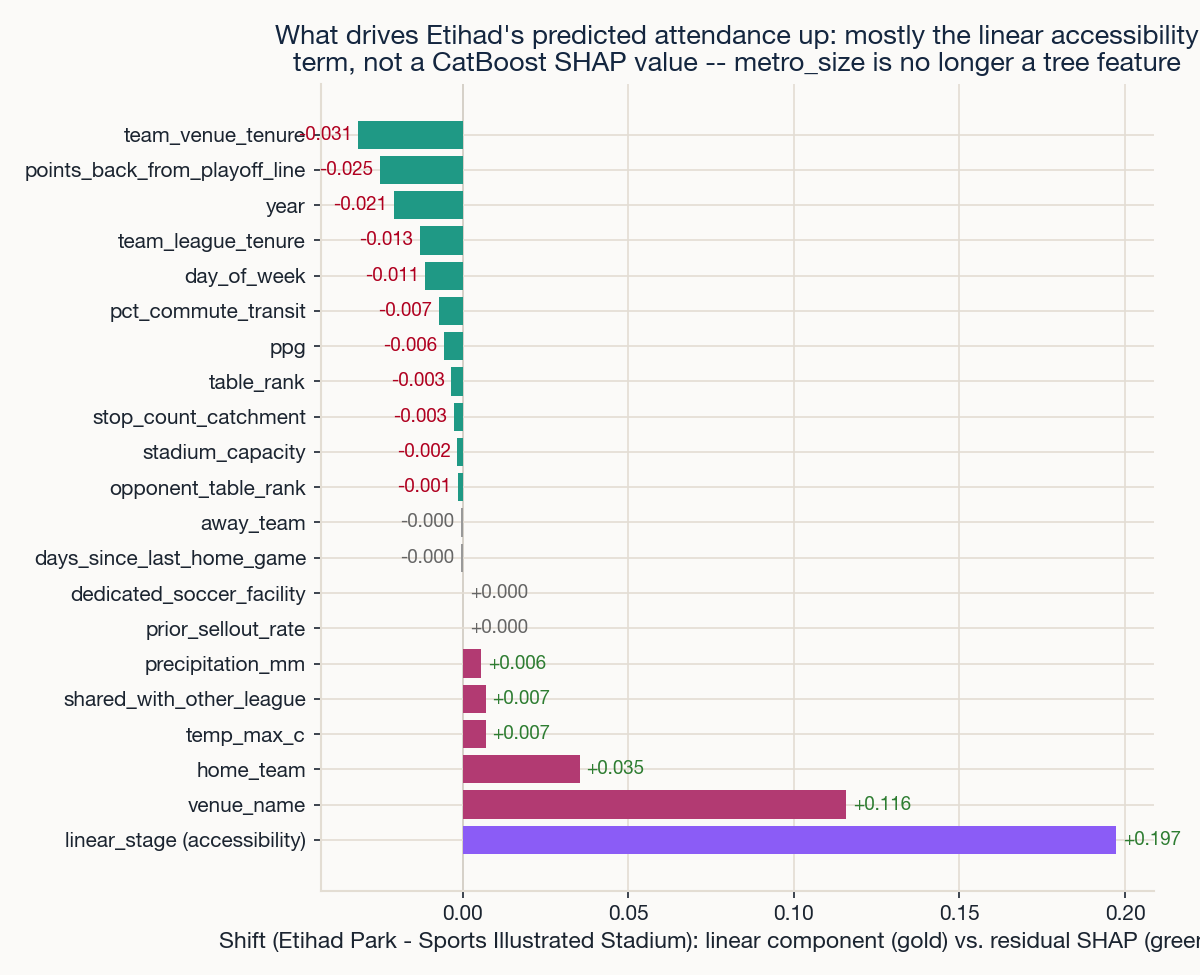
\includegraphics[width=0.5\linewidth]{shap_shift_diverging.png}
\caption{TreeSHAP decomposition of the predicted shift in log(attendance) from Sports Illustrated Stadium to Etihad Park, averaged across 54 paired synthetic rows. The linear accessibility term (purple) is the single largest contributor, ahead of venue and home-team recognition; every other residual feature contributes close to zero.}
\label{fig:shap2}
\end{figure}


\subsection{Synthetic control}
Table~\ref{tab:scm} shows Gotham FC's growth-corrected 2028 projection range. Without moving, by riding league-wide growth Gotham is projected to reach 10,926 fans (43.7 percent of capacity). Applying San Diego's growth-corrected relocation lift as a conservative scenario projects 14,962 fans (59.8 percent of capacity), while Seattle's growth-corrected lift projects 15,992 fans (64.0 percent of capacity), and Washington Spirit's growth-corrected lift projects 22,849 fans (91.4 percent of capacity).
\begin{table}[h!]
\centering
\caption{Projections for Gotham's first season at Etihad Park}
\begin{tabular}{@{}p{0.5\linewidth}p{0.22\linewidth}p{0.18\linewidth}@{}}
\toprule
Scenario & Projected att. & \% capacity \\
\midrule
No-move baseline (trend only) & 10,925.8 & 43.7\% \\
Etihad low (San Diego, corrected) & 14,961.5 & 59.8\% \\
Etihad mid (Seattle, corrected) & 15,991.6 & 64.0\% \\
Etihad high (Wash. Spirit, corrected) & 22,849.3 & 91.4\% \\
\bottomrule
\end{tabular}
\label{tab:scm}
\end{table}

\begin{figure}[h!]
\centering
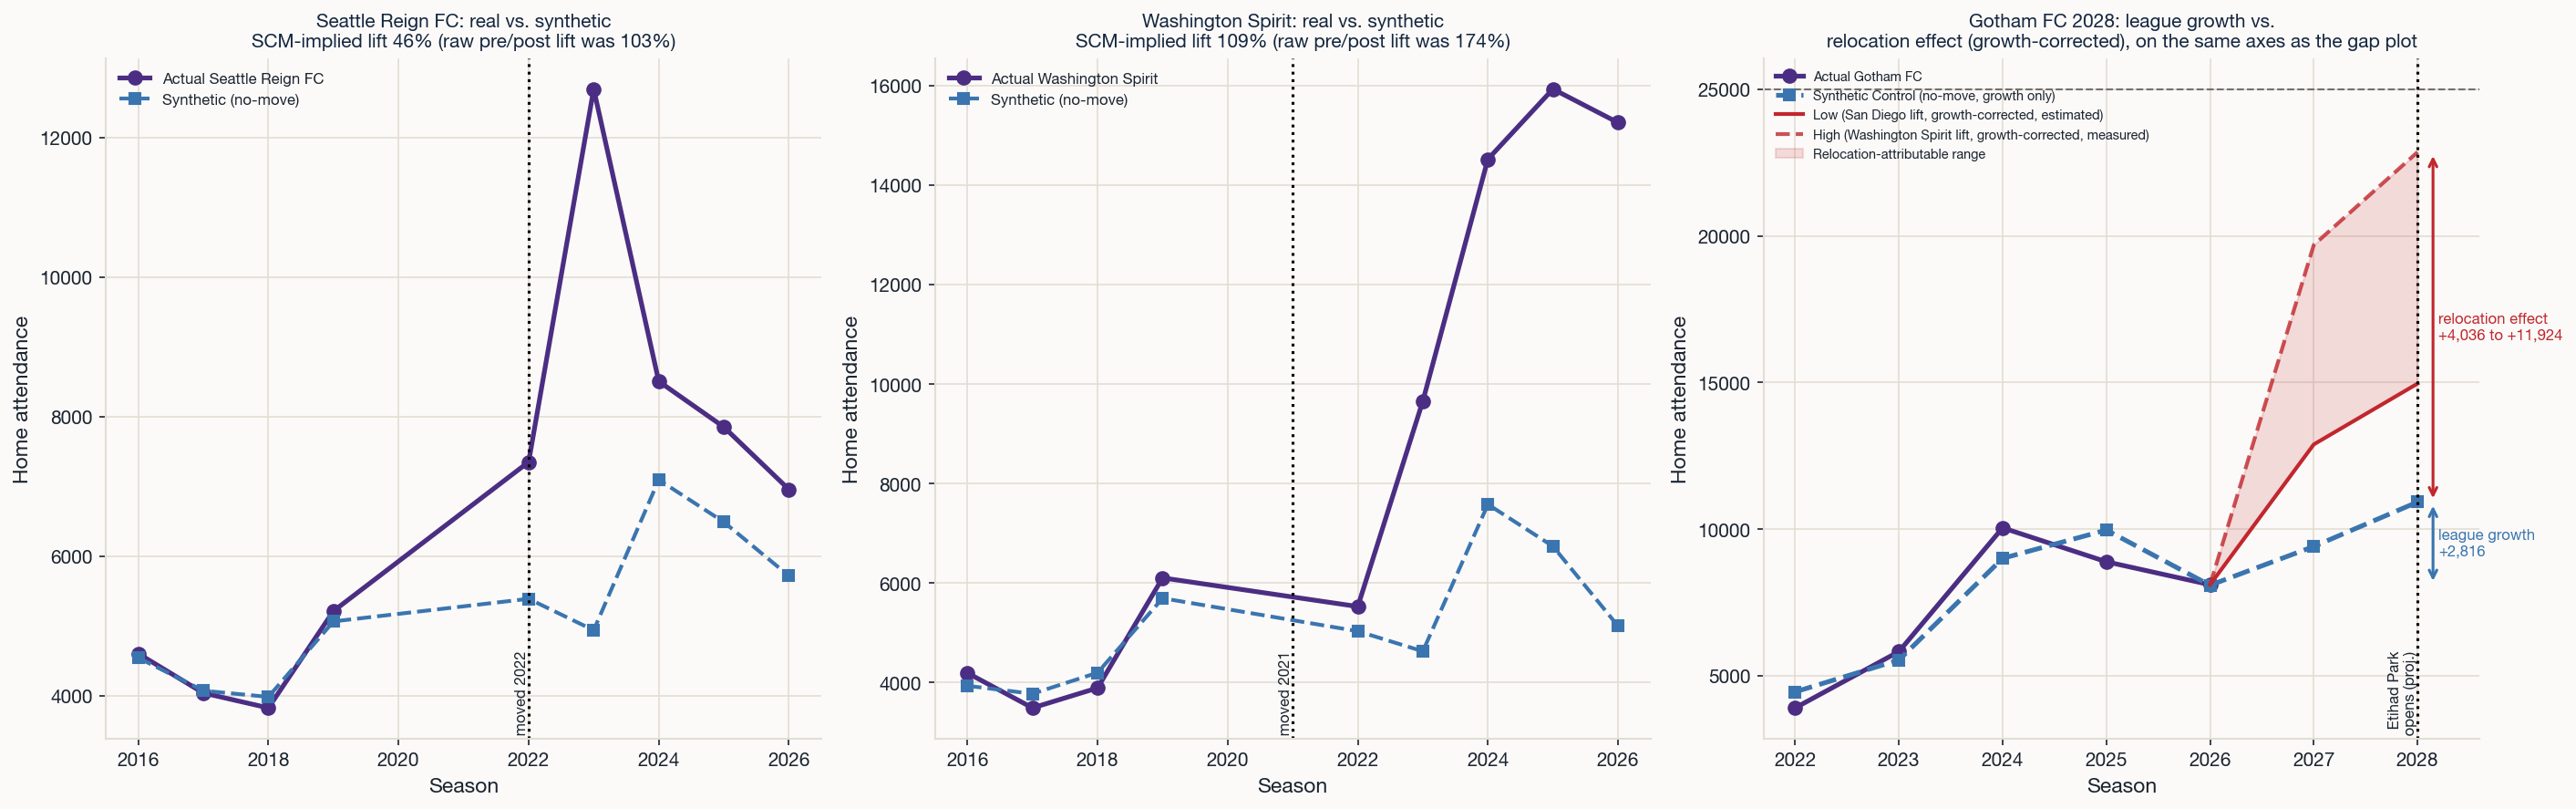
\includegraphics[width=0.8\linewidth]{synthetic_control_three_panel_summary.png}
\caption{Left, center: placebo validation of the synthetic-control design on the two comparable relocations that have already happened. Seattle Reign's raw pre/post lift is 103\% against an SCM-implied lift of 46\%; Washington Spirit's raw lift is 174\% against an SCM-implied lift of 109\%. Right: Gotham's own growth-corrected 2028 projection, decomposing the gap between the no-move synthetic control and the relocation scenarios into a league-growth component (+2,816) and a relocation-attributable component (+4,036 to +11,924).}
\label{fig:scm}
\end{figure}
The placebo validation on Seattle and Washington Spirit found rmspe ratios of 18.0 and 10.6 against their respective donor pools, but a permutation test placing Gotham's placebo alongside the other 4 donor teams' own placebo fits returns $p=0.2$ for both, not conventionally significant. With only 4 potential placebo units in the donor pool, this test cannot rule out that either result arose by chance, a direct consequence of how few comparable NWSL relocations currently exist.

\section*{Discussion}
Compared to the literature, these results suggest that the market-access model is true in the NWSL, rather than the enclosure model, since every estimate rewards gains in population reach, consistent with the suburban penalty \cite{DoesLocationMatterAnEconometricAnalysisofStadiumLocationandAttendanceatNationalWomensSoccerLeagueMatches}.My first hypothesis that the catchment population is positively associated with attendance across the league holds, as the linear coefficient is positive and significant. The second hypothesis that accessibility drives the relocation effect holds, but partially by design because accessibility enters through the linear stage. The last hypothesis that the size of the attendance lift tracks the size of the accessibility gain is consistent across the three relocations, but this is anecdotal and cannot be separated from the honeymoon effect.

The models consistently suggest that relocating to Etihad Park is likely a real driver of attendance growth, and accessibility is the most likely reason why. The growth-corrected range of 14,962–22,849 (60–91 percent of capacity) from synthetic control is our strongest estimate, corroborated by the CatBoost SHAP check, in which the linear accessibility term is the single largest driver of Etihad Park's predicted lift over Sports Illustrated Stadium. Every predictive model, however, struggled to generalize. The linear stage alone cannot beat a mean-only baseline on an unseen venue, and the much more feature-robust, tuned CatBoost residual model has a pooled LOVO $R^2$ of just 0.004. That is a significant increase from all other stages of model development for this project, but it still does not mean that the model can generalize to a stadium it has not seen before, like Etihad Park.

The synthetic control estimate is more reliable to produce an estimate for Gotham's attendance at Etihad Park, but it is constrained by a lack of data as only 4 teams have relocated in recent years, the pre-period fits are based on 4 years, and neither placebo reached conventional significance. The synthetic control model shows that stadium relocation increases attendance, but it does not isolate the effect of accessibility within that. The baseline used for synthetic control should be treated as a floor rather than a forecast, since it is based on 2026 growth, and does not account for 2027 growth for the sake of avoiding over-extrapolation.

This project has several constraints. There are only 4-5 recent NWSL relocations to learn from, and only 9 available seasons of data. The lack of data constrained this project, but it also means that no one knows the ceiling of the current growth of women's sports, which is why I set out on this project in the first place. I am looking forward to observing how Gotham's 2028 attendance actually plays out, and as more data becomes available over time, I hope to improve the model by separating the honeymoon effect of a new stadium from transit accessibility improvements specifically, and by testing whether one-off games in large venues, like Gotham FC's Citi Field game, are a reliable signal for teams considering a stadium move.

\section{Materials and methods}
Python was used for all of the analysis. Transit and walk isochrones were built with r5py 1.1.7 over each metro's GTFS feeds and clipped OpenStreetMap extracts, at a corrected walking speed of 5.0 km/hr, and joined to 2020 Census tract geometries and ACS demographics with geopandas 1.1.4. The linear accessibility stage was fit in statsmodels 0.14.6 with standard errors clustered by team, the residual stage in CatBoost 1.2.10, and the feature importance with SHAP 0.52.0 using TreeExplainer. Synthetic control weights were solved as a constrained least-squares problem with scipy 1.16.3. Game and attendance data come from the American Soccer Analysis API through the itscalledsoccer wrapper, and game-day weather from the Open-Meteo Archive API. All code, processed data, and figures are available at \url{https://github.com/isabelpt/nwsl-gotham-relocation}.

\section{Agentic analysis} Claude Code (Sonnet 5, Opus 5) was used to assist with elements of this analysis, and was especially useful for pulling GTFS feeds from 14 metro areas in a time-efficient manner. A detailed breakdown of what I accepted, what I rejected, and where it went wrong is available at this link \url{https://github.com/isabelpt/nwsl-gotham-relocation/blob/main/agentic_analysis.md}.


\section{References}
\bibliography{references}

\acknow{I would like to thank Professor Herbert Chang and my QSS 20 and 45 peers for their consultation, and Risa Isard, PhD, for her insights on the women's sports landscape.}

\showacknow % Display the acknowledgements section

% Bibliography


\end{document}
